\documentclass[shortabstract, english, lic]{iithesis}
\usepackage[utf8]{inputenc}
\usepackage{enumitem}
\usepackage{filecontents}
\usepackage{url}
\usepackage{breakcites}
\usepackage{graphicx}
\usepackage{caption}
\usepackage{subcaption}
\usepackage{tabularx}
\usepackage[T1]{fontenc}
\usepackage{titlesec}
\usepackage{amsthm}
\usepackage{amsmath}
\usepackage{amsfonts}
\usepackage{bbm}
\usepackage{float}
\usepackage{afterpage}
\usepackage{makecell}
\usepackage{multirow, fixltx2e}
\usepackage{algorithm}
\usepackage{algpseudocode}
\usepackage{hyperref}
\usepackage[rightcaption]{sidecap}
\usepackage[usenames, dvipsnames]{xcolor}
\usepackage[nottoc]{tocbibind}
\usepackage[section]{placeins}
\usepackage{bbm}
\usepackage[titles]{tocloft}

\graphicspath{{qualitative-results/}{quantitative-results/}}

\titleformat{\chapter}[block]{\normalfont\huge\bfseries}{\thechapter.}{5pt}{\huge}
\titlespacing*{\chapter}{0pt}{-19pt}{25pt}
\titleformat{\section}[block]{\normalfont\Large\bfseries}{\thesection.}{5pt}{\Large}
\titleformat{\subsection}[block]{\normalfont\large\bfseries}{\thesubsection.}{4pt}{\large}
\setlength{\cftbeforechapskip}{-2pt}

\DeclareMathOperator*{\argmax}{arg\,max}

\newcommand\blankpage{\null\thispagestyle{empty}\newpage}
\newcommand\numberedchapter[1]{\setlength\topskip{3cm}\chapter{#1}\setlength\topskip{0cm}}

\newtheoremstyle{default_theorem_style}
  {1em plus .2em minus .1em}%   Space above
  {1em plus .2em minus .1em}%   Space below
  {\slshape}%  Body font
  {}%          Indent amount (empty = no indent, \parindent = para indent)
  {\bfseries}% Thm head font
  {.}%         Punctuation after thm head
  {0.5em}%     Space after thm head: " " = normal interword space;
     %         \newline = linebreak
  {}%          Thm head spec (can be left empty, meaning `normal')


\theoremstyle{default_theorem_style}\newtheorem{theorem}{Theorem}
\theoremstyle{default_theorem_style}\newtheorem{definition}{Definition}

\polishtitle    {Gradientowy algorytm Metropolis-Hastings z zastosowaniami do odszumiania obrazów}
\englishtitle   {Gradient-based Metropolis-Hastings algorithm with applications to image denoising}
\author         {Dawid Wegner}
\advisor        {dr hab. Paweł Lorek}
\date           {29 sierpnia 2021}

\englishabstract{Markov chain Monte Carlo (MCMC) methods form a class of algorithms for sampling from a given
probability distribution.\ In particular, they proved to be effective when the state space is very large.\ In this
thesis we show how to leverage the above-mentioned methods to denoise binary images.\ Furthermore, we develop
gradient-based MCMC method and provide an efficient implementation that outperforms classic MCMC algorithms in terms of
denoising speed.\ Additionally, we present the results of our experiments, examining the performance of our method
depending on image size and noise level.\ Finally, we extend our approach to the case where some pixels of a grayscale
image are flipped, while showing that it generates near-perfect reconstructions of original images in relatively
low number of steps.}

\polishabstract{Próbkowanie Monte Carlo łańcuchami Markowa (MCMC) to klasa algorytmów służąca do próbkowania z danego
rozkładu prawdopodobieństwa.\ W szczególności okazały się one skuteczne w przypadkach, gdy przestrzeń stanów jest
bardzo duża.\ W poniższej pracy dyplomowej pokazujemy, jak wykorzystać powyższe metody do odszumiania obrazów
binarnych.\ Ponadto opracowujemy gradientową metodę MCMC oraz jej wydajną implementację, która przewyższa
klasyczne algorytmy MCMC pod względem szybkości odszumiania.\ Dodatkowo przedstawiamy wyniki naszych eksperymentów,
badających wydajność naszej metody w zależności od rozmiaru obrazu i poziomu szumu.\ Na koniec rozszerzamy nasze
podejście do przypadku, gdy niektóre piksele szarego obrazka są odwrócone, jednocześnie pokazując że nasza metoda
rekonstruuje oryginalne obrazki w stosunkowo niewielkiej liczbie kroków.}

\begin{document}

\numberedchapter{Introduction}

Markov chain Monte Carlo (MCMC) methods are used to simulate a random variable over a very large space.\ These
techniques have been successfully applied to many complex problems, like sampling graph colorings with given
probabilities.\ From the theoretical perspective, MCMC methods operate by constructing a Markov Chain, whose
stationary distribution matches a given target distribution to sample from.\ The ergodic theorem for Markov chains
states that under certain conditions, the constructed chain always converges to its stationary distribution.\ One
of the most known MCMC methods is known as the Metropolis-Hastings algorithm, whose the main component is the proposal
distribution used to transition to new states.\ In most applications, the proposal distribution is independent from
the target distribution.\ In this thesis, we propose to utilise gradient information contained in the target
distribution in order to increase the converge rate of simulated chains.\ While similar approach is taken in
\cite{oops_gradient}, we put more effort into how to implement this method efficiently for sparse graphs.\newline

\noindent One of the main challenges in Computer Vision is the image denoising problem, in which the goal is to
reconstruct an original image given its noisy version.\ The considered problem plays an important role in the area
of image retrieval as the noise is present in many practical situations e.g.\ on photos taken with cameras.\ Moreover,
the noise cannot be removed using simple heuristics.\ While many sophisticated approaches have been already proposed
to solve the stated problem, it remains an open area of research.\ In this thesis, we tackle the problem of image
denoising using the developed MCMC method.\ Additionally, we provide an efficient implementation of our
method in Python.

\numberedchapter{Markov chains}

In this chapter we will formally define the notion of Markov chain and list its basic properties.\ Particularly,
we will characterise a stationary distribution and reversible Markov chains.\ These tools are necessary to understand
the theory behind Markov chain Monte Carlo methods that are discussed in \textit{Chapter} \ref{chapter:mcmc}.

\section{Basic properties}

Formally, a Markov chain is a stochastic process in which the probability of the next event depends only on the current
state.\ Intuitively, we can think of such process as a directed graph with loops.\ An example of a Markov chain that
describes weather conditions is shown in Figure \ref{fig:markov_chain}.\ In this case, our state space contains three
elements: $\{Sunny,\ Cloudy,\ Rainy\}$.\ Each directed edge represents the probability of transitioning from a state
$X_k$ to a state $X_{k + 1}$.\ In the example presented in Figure \ref{fig:markov_chain}, the probability that the
weather will be \textit{rainy} on the day $X_{k + 1}$, conditioned on the fact that it was \textit{cloudy} on the
day $X_k$, is equal to $0.5$.\ Note that the described process carries an underlying assumption that the weather in
the next day depends only on the weather in the present day.\newline

\begin{figure}[H]
\centering
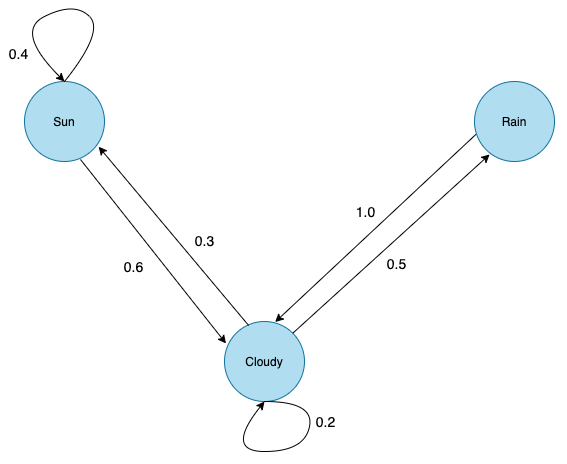
\includegraphics[scale=0.43]{markov_chain}
\caption{An example of a Markov chain describing weather conditions.}
\label{fig:markov_chain}
\end{figure}

\noindent Although a Markov chain can contain infinitely many states, we only consider
the ones with a finite number of them.\ In particular, some theorems presented in the next sections
are not true without this assumption.\ The graph representation of a Markov chain is useful, but in most cases
it's convenient to think of it as a matrix.\ Formally, let us define an element $0 \leq P_{ij} \leq 1$ of a matrix
$P$ as the probability of transitioning from the state $i$ to the state $j$.\ As the $i$-th row of such matrix
defines probabilities of transitioning from the $i$-th  state to all other states, the equality
$\sum_{j = 1}^{n} P_{ij} = 1$ holds.\ A matrix with the above-mentioned properties is called a
\textit{stochastic} matrix.\ In the next sections, we will think of a Markov chain in this way.

\begin{definition}
A vector $\mu^{(0)} = (\mu^{(0)}_1, \mu^{(0)}_2, \dots, \mu^{(0)}_n)$ such that $\sum_{i=1}^{n} \mu^{(0)}_i = 1$
is called an \textit{initial distribution} of a Markov chain.\ It defines an initial distribution across the state space.

\end{definition}

\noindent The Markov chain process is fully characterized by its transition matrix $P$ and an initial
distribution $\mu^{(0)}$.\ In particular, the distribution of a Markov chain in the $k$-th step can be uniquely
determined i.e.\ the equality $\mu^{(k)} = \mu^{(0)}P^k$ holds.

\section{Stationary distribution}

In this section we will formalize the notion of stationary distribution and explore its properties.\ Furthermore,
we will provide sufficient conditions to guarantee that a Markov chain has a unique stationary distribution.

\begin{definition}
A probability distribution $\pi = (\pi_1, \pi_2, \dots, \pi_n)$ is called a \textit{stationary} distribution if and only if
$\pi P = \pi$, where $P$ denotes a transition matrix of a Markov chain.
\end{definition}

\noindent One can convince yourself that a Markov chain can have multiple stationary distributions.\ An example of
such Markov Chain is when $P = Id$, which implies that any probability distribution is stationary.

\begin{definition}
A Markov chain with a transition matrix $P$ is called \textit{irreducible} if and only if for each pair of the source
state $i$ and the destination state $j$, it's possible to transition from $i$ to $j$ in a finite time i.e.\ there
exists $k$ such that $(P^k)_{ij} > 0$.
\end{definition}

\begin{definition}
A period of the $i$-th state is defined as $p(i) = gcd(\{n \geq 1 : (P^n)_{ii} > 0\}$.\ A state is called
\textit{aperiodic} if $p(i) = 1$.\ A Markov chain is called aperiodic if all of its states are aperiodic.
\end{definition}

\noindent A Markov chain that respects the two above-mentioned properties is called an \textit{ergodic} Markov
Chain.\ Interestingly, ergodic Markov chains have many useful properties that lead to sophisticated algorithms.

\begin{theorem}\label{thm:one_stationary}
For any ergodic Markov chain, there exists exactly one stationary distribution $\pi$.
\end{theorem}

\begin{theorem}\label{thm:converges_to_stationary}
Let $\mu^{(0)}$ be an arbitrary initial distribution of any ergodic Markov chain.\ Let
$d_{TV}(\mu^{(n)}, \pi) = \frac{1}{2} \sum_{i = 1}^{k} |\mu_i^{(n)} - \pi_i|$ denote a distance between a
distribution of possible states in the $n$-th step and a stationary distribution of the defined Markov chain.\ Then,
the equality $\lim_{n \to \infty} d_{TV}(\mu^{(n)}, \pi) = 0$ holds.
\end{theorem}

\noindent The proofs of \textit{Theorem} \ref{thm:one_stationary} and \textit{Theorem}
\ref{thm:converges_to_stationary} can be found in \cite{markov_chains_book}.\ From the practical point of view, the
presented theorems imply that an ergodic Markov chain always converges to its stationary distribution, regardless of
the initial distribution.\ Note that the presented theorems do not guarantee any convergence speed.

\section{Reversible Markov chains}

Reversible Markov chains show up in many different areas e.g.\ they are the main building block for the Markov
Chain Monte Carlo methods.\ They are called this way as they look the same regardless of whether time runs
backwards or forwards.

\begin{definition}
A probability distribution $\tilde{\pi}$ is said to be \textit{reversible} for a Markov chain with a transition
matrix $P$ if and only if for any $i,j$ it holds $\tilde{\pi_i} P_{ij} = \tilde{\pi_j} P_{ji}$.\ A Markov chain is called
reversible if there exists a reversible distribution $\tilde{\pi}$ for it.
\end{definition}

\begin{theorem}\label{reversible_chain}
If a Markov chain is reversible with the distribution $\tilde{\pi}$, then $\tilde{\pi}$ is a stationary distribution
i.e.\ $\tilde{\pi} = \pi$.
\end{theorem}

\begin{proof}
Using the fact that each row of $P$ sums to $1.0$, we have
$$
(\tilde{\pi} P)_j = \sum\limits_i \tilde{\pi}_i P_{ij} = \sum\limits_i \tilde{\pi}_j P_{ji} =
\tilde{\pi}_j \sum\limits_i P_{ji} = \tilde{\pi}_j\ .
$$
\end{proof}

\noindent The presented theory has many useful implications.\ First of all, in order to determine
whether a distribution is reversible, it suffices to check if it exists a probability measure $\tilde{\pi}$ such that
for any $i, j$ the equality $\tilde{\pi_i} P_{ij} = \tilde{\pi_j} P_{ji}$ holds.\ What is more, in case we find such
$\tilde{\pi}$, it follows that $\pi = \tilde{\pi}$ i.e.\ the probability measure that we found is a stationary
distribution.\ As a result, this equation gives us a powerful tool for finding a stationary distribution.

\numberedchapter{Markov chain Monte Carlo methods}\label{chapter:mcmc}

Consider a problem of sampling a random permutation from the set of $100$ elements.\ One can show that such space
contains $100!$ elements, implying that putting all permutations in the memory of a computer is not feasible.\ While
there exists algorithms for sampling permutations from a uniform distribution, the problem becomes harder in the case of
a skewed distribution.\ For instance, let our target distribution be defined based on positions of permutation's
elements e.g.
$$
d(x) = \frac{\prod_{i = 1}^{n} e^{i \cdot x_i}}{Z}\ ,
$$
where $x_i$ denotes the $i$-th element of the permutation and $Z$ is the normalising constant.\ While the problem
of sampling from such distribution can not be tackled using any trivial algorithm, it's possible to simulate the
sampling process with Markov chains.\newline

\noindent In this chapter, we will show how to deal with a situation in which we have a large state space and our
task is to sample an element from this space effectively.\ We will leverage the theory presented in the previous
section to show how to construct a Markov chain with a stationary distribution equal to the target distribution we
want to sample from.

\section{Metropolis–Hastings algorithm}

Let us denote the target distribution we want to sample from as $\tilde{\pi}$.\ Notice that in order to produce samples
from $\tilde{\pi}$ one may construct a Markov chain $X$ with a transition matrix $P$ and a stationary distribution
$\pi = \tilde{\pi}$.\ As a result, it suffices to simulate $X$ until we reach the stationary distribution.\ Assuming
that $X$ is ergodic, it can start in any initial distribution and based on \textit{Theorem} \ref{thm:converges_to_stationary}
it is guaranteed to converge to $\pi$.\ As one of our assumptions says that the space of states is very large,
constructing such Markov chain explicitly does not solve our problem.\newline

\noindent Before presenting the full algorithm, we will show how to construct a matrix $P$ such that $\tilde{\pi}$ is a
stationary distribution of a Markov chain $X$ corresponding to $P$.\ Let us assume that we have some proposal
distribution $Q$ that defines a transition matrix of a Markov chain with the same state space as $X$.\ Going further,
let us define a matrix $P$:\newline
$$
P_{ij} =
\begin{cases}
  Q_{ij}\min{(1, \frac{\pi_j Q_{ji}}{\pi_i Q_{ij}})} &\text{if $i \ne j$}\\
  1 - \sum\limits_{k \ne i}Q_{ik} \min{(1, \frac{\pi_k Q_{ki}}{\pi_i Q_{ik}})} &\text{otherwise}
\end{cases}\ .
$$

\noindent While at first it may be unintuitive why $P$ would have a stationary distribution $\pi$, it can be easily
proved.\ To do so, let us show that for any $i, j$ the equality $\pi_i P_{ij} = \pi_j P_{ji}$ holds.\ Without
any loss of generality, we can assume that $\frac{\pi_j Q_{ji}}{\pi_i Q_{ij}} \leq 1$, which implies that
$\frac{\pi_i Q_{ij}}{\pi_j Q_{ji}} \geq 1$.\ Putting everything together, we get
$$
\pi_i P_{ij} = \pi_i Q_{ij} \frac{\pi_j Q_{ji}}{\pi_i Q_{ij}} = \pi_j Q_{ji} = \pi_j P_{ji}\ ,
$$
which proves that $\pi_i P_{ij} = \pi_j P_{ji}$.\ The case when $\frac{\pi_j Q_{ji}}{\pi_i Q_{ij}} \geq 1$ is
symmetric.\ Using \textit{Theorem} \ref{reversible_chain}, we can conclude that $\pi$ is the stationary distribution
of the constructed Markov chain.\newline

\noindent Equipped with the method for generating a transition matrix $P$ for a given stationary distribution $\pi$,
one may construct an algorithm \ref{alg:metropolis_hastings} simulating a Markov chain that corresponds to $P$.\ In
case the proposal distribution $Q$ is symmetric (i.e.\ $Q_{ij} = Q_{ji}$), the presented algorithm is called the
\textit{Metropolis} algorithm, while in the general case of non-symmetric $Q$ it is called the
\textit{Metropolis-Hastings} algorithm.


\begin{algorithm}[tb]
\caption{Metropolis-Hastings}\label{alg:metropolis_hastings}
\begin{algorithmic}[1]
\State{\textbf{Input:} proposal distribution $Q$}
\State{\textbf{Input:} the current state $X_k = i$, where $k$ denotes the latest step of the simulation}
\State{Sample $j$ from a distribution $Q_i = (Q_{i1}, Q_{i2}, \dots, Q_{iN})$}
\State{Let $p = \min{(1, \frac{\pi_j Q_{ji}}{\pi_i Q_{ij}})}$}
\State{Sample $U \sim Unif(0, 1)$}
\If{$U \leq p$}
    \State{Set $X_{k + 1}$ = j}
\Else
    \State{Set $X_{k + 1} = X_k$}
\EndIf
\State{\textbf{Output:} the next state $X_{k + 1}$}
\end{algorithmic}
\end{algorithm}

\section{Gibbs sampling}\label{sec:gibbs_sampling}

\noindent In this section we will show how to simulate Markov chains for some specific distributions.\ Specifically,
let us assume that each possible state in a given state space can be represented by a function $e_i : V \to S$ that
maps each vertex $v \in V$ of an underlying graph $G = (V, K)$ to one of possible values $s \in S$.\ Generally, a state
that is represented in this form is often called a \textit{configuration}.\ While for some distributions this
representation may not make sense, there are multiple cases for which it is the most natural way of expressing a
given distribution.\ For instance, consider a problem of colouring a graph.\ In this case, each state corresponds to a
possible graph colouring i.e.\ each vertex $v \in V$ is assigned one colour $s \in S$.\newline

\noindent Now, assume that we are given a \textit{potential} function $H : E \to \mathbb R_{\geq 0}$ that assigns an
unnormalised probability to each configuration $e \in E$ i.e.\
$$
\pi(e) = \frac{H(e)}{Z}\ ,
$$
where $Z$ is the normalising constant.\ Our goal is to sample configurations with probabilities given by $\pi$.\ Let
us show how to simulate a Markov chain satisfying this condition.\ To
perform the $(k + 1)$-th step of the algorithm, assuming that the current state is equal to
$X_k = e_i$, first draw a vertex $\tilde{v} \in V$ uniformly and for each $s \in S$ calculate the probability
$$
P(J(\tilde{v}) = s\ |\ J(-\tilde{v})=e_i(-\tilde{v})) = \frac{\pi_{e(\tilde{v}) =
s,e(-\tilde{v}) = e_i(-\tilde{v})}}{\sum_{s' \in S} \pi_{e(\tilde{v}) = s', e(-\tilde{v}) = e_i(-\tilde{v})}}\ ,
$$
where $J \sim \pi$ is a random variable, $e(\tilde{v})$ refers to $s \in S$ assigned to the vertex $\tilde{v} \in V$
and $e(-\tilde{v})$ denotes assignments of $s \in S$ to vertices $v \in V \setminus \{\tilde{v}\}$.\ The last step of
the algorithm involves sampling $\tilde{s} \in S$ from the probability distribution
$P(J(\tilde{v}) = s\ |\ J(-\tilde{v})=e_i(-\tilde{v}))$ and setting
$$
X_{k + 1}(v) =
\begin{cases}
  \tilde{s} &\text{if $v = \tilde{v}$}\\
  X_k(v) &\text{otherwise}
\end{cases}\ .
$$

\noindent The presented \textit{Gibbs sampling} algorithm is a special case of the Metropolis-Hastings algorithm
with the proposal distribution
$$
Q_{ij} =
\begin{cases}
  \frac{1}{Z} &\text{iff $i$ is adjacent to $j$}\\
  0 &\text{otherwise}
\end{cases}\ ,
$$
which provides an instant proof of the the fact that the presented algorithm simulates a Markov chain with the
stationary distribution $\pi$.\ An alternative proof of this fact can be found in \cite{mcmc_book}.\ The advantage of
the $Gibbs$ algorithm over the $Metropolis$-$Hastings$ algorithm is that it avoids constructing  the proposal
distribution $Q$.\ At the same time, for some cases the lack of control over $Q$ is a major downside as we will see
in the following chapters.

\numberedchapter{Ising model and its applications}\label{chapter:ising_model}

\noindent In the present chapter we will discuss the \textit{Ising model} that is used by physicists to describe phase
transitions.\ While it may seem unrelated to the topic of image denoising, it turns out that the described model
can operate on any graph.\ In particular, we will show how to interpret images as graphs and apply the Ising model to
the problems of binary and grayscale image denoising.

\section{Formal definition of the Ising model}

In this section we will follow the notions introduced in \textit{Section} \ref{sec:gibbs_sampling}.\ Let us consider
a graph $G = (V, K)$ and a set $S = \{-1, 1\}$.\ Now, define a configuration $e_i : V \to S$ as a function that
maps vertices of $G$ to elements from $S$, and a potential function
$$
H(e_i) = \prod\limits_{(j, k) \in K} e^{\beta e_i(v_j)e_i(v_k)}\ ,
$$
where $\beta$ is a parameter that controls the strength of $coupling$ between vertices.\ The described model
is called the $Ising$ model.\ In physics, the elements $\{-1, \, 1\}$ of the set $S$ are interpreted as a negative and a
positive \textit{spin} respectively.\ Assuming that $\beta > 0$, the model assigns high probabilities to configurations
having the same spins assigned for neighbouring vertices.\ Note that the Ising model is uniquely determined for
a given graph $G$ and a parameter $\beta$.

\section{Applying MCMC methods to the Ising model}

Let us assume that we are given the Ising model represented by the potential function
$H : E \to \mathbb R_{\geq 0}$.\ Our goal is to produce samples from a probability distribution $\pi$ defined by
the formula
$$
\pi(e) = \frac{H(e)}{Z}\ ,
$$
where $Z$ is the normalising constant.\ One way of approaching this problem is to utilise MCMC methods described in
the $Chapter$ \ref{chapter:mcmc}.\newline

\noindent As we already described how to construct configurations for our model, the first algorithm that comes to mind
is the Gibbs sampler introduced in the $Section$ \ref{sec:gibbs_sampling}.\ Actually, it suffices to derive a formula
for the conditional probability $P(J(\tilde{v}) = s\ |\ J(-\tilde{v})=e_i(-\tilde{v}))$ for any $e_i \in E$,
$\tilde{v} \in V$ and $s \in \{-1,\ 1\}$, where $J \sim \pi$.\ By expanding and simplifying this expression, we get
$$
P(J(\tilde{v}) = -1\ |\ J(-\tilde{v})=e_i(-\tilde{v})) =
\frac{\pi_{e(\tilde{v}) =
-1,e(-\tilde{v}) = e_i(-\tilde{v})}}
{\sum\limits_{s' \in \{-1, 1\}} \pi_{e(\tilde{v}) = s', e(-\tilde{v}) = e_i(-\tilde{v})}} =
\frac{1}{1 + 2 \sum\limits_{(\tilde{v}, \tilde{w}) \in K} e_i(\tilde{w})}
$$
and utilising the fact that $|S| = 2$
$$
P(J(\tilde{v}) = 1\ |\ J(-\tilde{v})=e_i(-\tilde{v})) = 1 - P(J(\tilde{v}) = -1\ |\ J(-\tilde{v})=e_i(-\tilde{v}))\ .
$$

\noindent As we just have shown, the problem of updating the spin of a vertex $\tilde{v}$ reduces to the computation of
neighbours' spins.\ Furthermore, the derived formula can be calculated efficiently in the time
complexity $\mathcal{O}(1)$ as one may store and update the information about the sum of neighbours'
spins for each $v \in V$.\newline

\noindent It is easy to convince yourself that the Metropolis-Hastings algorithm can be applied to the Ising model
too.\ To do so, one needs to come up with the proposal distribution $Q$ and be able to calculate the expression
$\min{(1, \frac{\pi_j Q_{ji}}{\pi_i Q_{ij}})}$ for each $i, j \in E$.\ If we define the neighbourhood of configurations
similarly as it is defined in the Gibbs sampler, the considered expression will simplify considerably. \ The
advantage of this approach is that we can construct $Q$ in a way that the simulated chain will converge faster.\newline

\noindent The final question is why do we care about sampling from the Ising model?\ To answer this question, one may
observe that some configurations are assigned much higher probability than the others.\ It means that when the simulated
Markov chain will converge to its stationary distribution, it will start producing samples that have very high
potential according to the function $H$.\ Actually, the most common application of the Ising model is to find
those configurations that have a high probability while rejecting the others.\ In particular, if we add
additional constraints, the problem of maximising the potential function is not trivial.

\section{Application to binary image denoising problem} \label{sec:binary_images_problem}

Consider a problem in which we are given a binary image with some pixels flipped.\ Formally, let denote a coordinate
$(i, j)$ of our observation by $\tilde{Z}_{ij} \in \{0, 255\}$.\ The goal is to find an original image $X$ such that
$X_{ij} \in \{0, 255\}$, leveraging the fact that $\tilde{Z}$ was constructed using the following formula
$$
\tilde{Z}_{ij} =
\begin{cases}
  255 - X_{ij} &\text{if $U_{ij} < \alpha$}\\
  X_{ij} &\text{otherwise}
\end{cases}\ ,
$$
where $U_{ij}$ is an i.i.d.\ sequence of $Unif(0, 1)$ random variables.\newline

\noindent As we are interested in images representing real objects, we can safely assume that most of the neighbouring
pixels should have the same value.\ Combining it with the fact that $\tilde{Z}$ was generated by flipping pixels of
$X$ with some unknown probability $\alpha$, we can construct a model that finds $X$ providing the best balance between the
two above-mentioned constraints.\newline

\noindent Now, let us think of images as graphs in which the neighbourhood of a vertex representing a
coordinate $(i, j)$ is defined as $\{(i - 1, j), (i + 1, j), (i, j - 1), (i, j + 1)\}$.\ In
order to have it properly defined for pixels in the corners on an image, one may add margins.\ Additionally, to keep
the following formulas simple, let us assume that each coordinate $(i, j)$ corresponds to some
vertex $v_k$, forming the graph $G = (E, K)$.\ Formally, for each pair $(i, j)$, there exist
$k \in \mathbb{N}$, such that $v_k = (i, j)$.\ Now, define $S = \{-1, 1\}$ and map our pixels by applying the
following function
$$
\hat{Z}_{ij} =
\begin{cases}
  -1 &\text{if $\tilde{Z}_{ij} = 0$}\\
  1 &\text{if $\tilde{Z}_{ij} = 255$}
\end{cases}\ .
$$

\noindent The described model is the Ising model that assures that neighbouring pixels have the same values.\ In order
to take into account the second constraint, one may increase the potential of configurations that have their pixel
values equal to the observed values defined by $\tilde{Z}$.\ Putting it all together, we get the following potential
function:
$$
H(e_i) = \prod\limits_{(j, k) \in K} e^{\beta e_i(v_j)e_i(v_k)}
\prod\limits_{j \in V}(\mathbbm{1}_{e_i(v_j) = \hat{Z}(v_j)}(1 - \alpha) +
\mathbbm{1}_{e_i(v_j) \neq \hat{Z}(v_j)}\alpha)\ ,
$$
where $1 - \alpha, \beta$ are the parameters controlling the observation strength and the coupling strength
respectively.\ Intuitively, increasing the observation strength causes our model to put less weight to the
observed pixels in $\tilde{Z}$, while increasing the coupling strength enforces the neighbouring pixels to have the
same values.

\section{Extension to grayscale images}

In the present section we will show how to extend the model described in \textit{Section}
\ref{sec:binary_images_problem} to grayscale images.\ Formally, given an observation $\tilde{Z}$ such
that $\tilde{Z}_{ij} \in \{0, 1, \dots, 255\}$ the goal is to find an original image $X$.\ In this paper, we assume
that $\tilde{Z}$ was generated by flipping random pixels of $X$ i.e.
$$
\tilde{Z}_{ij} =
\begin{cases}
  255 - X_{ij} &\text{if $U_{ij} < \tilde{\alpha}$}\\
  X_{ij} &\text{otherwise}
\end{cases}\ ,
$$
where $U_{ij}$ is an i.i.d.\ sequence of $Unif(0, 1)$ random variables.\ We leave more general case for the future
work.\ Similarly to the case of binary images, our optimization goal is to maximise the potential function that
takes into account the observation $\tilde{Z}$ and the coupling between neighbouring pixels.\ While there are many
ways to define such potential function $H$, we find that the following function
$$
H(e_i) = \prod\limits_{(j, k) \in K} e^{-\beta |e_i(v_j) - e_i(v_k)|}
\prod\limits_{j \in V}(\mathbbm{1}_{e_i(v_j) = \tilde{Z}(v_j)}(1 - \alpha) +
\mathbbm{1}_{e_i(v_j) \neq \tilde{Z}(v_j)}\alpha)
$$
expresses our constraints in efficient and intuitive way.\ In particular, the penalty given by the coupling part of
the function $H$ is proportional to the sum of distances between a considered pixel and all its neighbours.\ As a
result, the model is encouraged to flip those pixels that are significantly different from all of its
neighbours.\ The other characteristic of the function $H$ is that for the neighbouring configurations, most of
components of the coupling product are equal, making the update rule of the Gibbs algorithm simple and efficient.

\numberedchapter{Gradient-based image denoising}

Although we have shown how to remove noise from images using Gibbs sampling, we still lack an efficient algorithm
that would denoise images in a low number of steps.\ In order to convince yourself that the presented method
might perform many unnecessary steps, recall that it samples $v \in V$ in each step uniformly.\ From the perspective
of our problem, it means that each pixel has the same probability of being chosen and potentially updated.\ While
it may be an effective approach at the beginning of the denoising process, closer to the end of the process there is
very little chance to sample a pixel that should be updated.\newline

\noindent This issue motivates our gradient-based approach
that will be discussed in the present chapter.\ While a similar approach is taken in \cite{oops_gradient}, we put
more effort into how this method can be implemented efficiently for sparse graphs, showing how to perform one
step of the presented algorithm in the time complexity $\mathcal{O}(1)$.

\section{Proposal distribution inspired by gradients}

In \textit{Chapter} \ref{chapter:ising_model} we have shown how to sample high-potential configurations by
utilising MCMC methods.\ While this approach effectively approximates the stationary distribution of the constructed
Markov chain, our final goal is to find $\tilde{x} = \argmax_x H(x)$.\ In the case of continuous functions, such problem
is often tackled by computing a gradient of a given function $f(x^{(k)})$ with respect to the current state $x^{(k)}$.
Then, a small step is taken in the direction given by the gradient
i.e.\ $x^{(k + 1)} = x^{(k)} + \gamma \nabla f(x^{(k)})$, where $\gamma$ is a parameter
controlling the size of the step.\ The method is repeated many times until it converges to the local/global optima of
the given function $f$.\newline

\noindent In our scenario, $x$ represents an $n \times m$ image, which we can think of as a point in
$M = n \times m$ dimensional space.\ As the space of images is discrete, the above-discussed gradient update rule
cannot be applied directly.\ Nevertheless, the gradient of the function $H(x)$ with respect to the vector $x$ exists
and the information contained in it can be treated as a hint on which direction should be followed.\ A toy example
illustrating this intuition is shown in $Figure$ \ref{fig:gradient_example}.\newline

\noindent We propose to utilise the gradient information to construct the probability distribution over the
neighbours of the current state and update the state according to the constructed distribution.\ Specifically, let
us assume that the goal is to find an optimal image $\tilde{x}$ according to some function $\tilde{H}(x)$.\ At each
step, assuming that the current state is denoted by $x^{(k)}$, we sample a dimension (aka pixel number) $D$
following the distribution
$$
P(D = i) = \frac{e^{|(\nabla \tilde{H}(x^{(k)}))_i|}}{\sum\limits_{j = 1}^{n}
e^{|(\nabla \tilde{H}(x^{(k)}))_j|}} = softmax(|\nabla \tilde{H}(x^{(k)})|)
$$
and construct the next state $x^{(k + 1)}$ by increasing/decreasing the value of
$x^{(k)}_D$ (in a way that we stay in our discrete domain) based on whether $(\nabla f(x^{(k)}))_D$ is
positive/negative.\ For the remaining dimensions $i \neq D$, we copy the values from
$x^{(k)}$ i.e.\ we set $x^{(k + 1)}_i = x^{(k)}_i$.\ Intuitively, all neighbours of the state $x^{(k)}$
differ in exactly one dimension (aka pixel) from $x^{(k)}$ and in each step we choose which dimension
should be updated guided by the gradient of $\tilde{H}(x^{(k)})$.\newline

\begin{figure}[t]
\centering
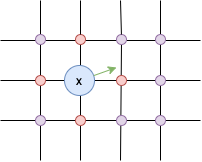
\includegraphics[scale=0.9]{gradient_example}
\caption{An example of how the gradient of $\tilde{H}(x)$ with respect to the current state $x^{(k)}$ (marked in green)
can be leveraged to pick the next state $x^{(k + 1)}$, iteratively converging to $\argmax_x \tilde{H}(x)$.\ In this
case, the gradient (green arrow) of the function $\tilde{H}(x)$ strongly points to the neighbour on the right side
of the current state and slightly to the top neighbour.\ Based on this, we expect our method to choose the right
neighbour as the next state $x^{(k + 1)}$ with a very high probability, while the top neighbour should be picked with
the significantly less probability and other neighbours should be ignored.}
\label{fig:gradient_example}
\end{figure}

\noindent Now, we will show how to derive the update rule for the image denoising problem.\ Recall that the Ising model
for our problem is defined by the potential function
$$
H(e_i) = H(x) = \prod\limits_{(j, k) \in K} e^{\beta x(v_j)x(v_k)}
\prod\limits_{j \in V}( \mathbbm{1}_{x(v_j) = \tilde{Z}(v_j)}(1 - \alpha) +
\mathbbm{1}_{x(v_j) \neq \tilde{Z}(v_j)}\alpha)\ ,
$$
where each coordinate $(i, j)$ of an image corresponds to some vertex $v_k$, forming the graph $G = (E, K)$.\ This
formula can be transformed to the more general form
$$
H(x) = e^{x^T W x} = e^{\tilde{H}(x)}\ ,
$$
where $W$ is $n \times n$ matrix encoding the observation and the coupling components of the potential
function.\ Particularly, in this case $W$ is an adjacency matrix of the graph $G = (E, K)$ scaled by the parameter
$\beta$, except for the diagonal elements for which either $W_{ii} = ln(\alpha)$ or $W_{ii} = ln(1 - \alpha)$.\ In
this formulation, the goal is to find $\argmax_x \tilde{H}(x) = x^T W x$.\ Taking the gradient of
$\tilde{H}(x)$ with respect to $x$, we get
$$
(\nabla \tilde{H}(x))_i = (2W x)_i = \sum_{i, j} W_{ij} x_j\ ,
$$
which enables us to sample a neighbour of $x$ according to the probability distribution
$softmax(|\nabla \tilde{H}(x)|)$.\ Interestingly, we may interpret this process as a one step of the
Metropolis-Hastings algorithm with the proposal distribution
$$
Q_x = softmax(|\nabla \tilde{H}(x)|)\ ,
$$
which implies that in order perform our gradient-based update rule, one may use already developed
\textit{Algorithm} \ref{alg:metropolis_hastings}.\ Furthermore, the developed proposal distribution is simple,
particularly for each dimension (aka pixel) the developed formula contains only the neighbouring
dimensions (aka pixels).

\section{Efficient implementation for image denoising}\label{sec:efficient_denoising}

While the developed gradient-based method provides a way to find pixels that should be updated, the naive
implementation performs one step of the algorithm in the time complexity $\mathcal{O}(M)$,
where $M$ denotes the number of pixels of a given image.\ In contrast, the Gibbs
algorithm provides the time complexity $\mathcal{O}(1)$ of one step, which means that it can update
$\mathcal{O}(M)$ random pixels while our method would update only one pixel in the same time.\ This issue makes
our method not scalable for high-resolution images.\ In this section, we will show how to reduce the complexity
of our algorithm to $\mathcal{O}(1)$, making it efficient for high-dimensional images.\newline

\noindent Let us assume that the simulated chain is in the state $x^{(k)}$ and we have already constructed the
proposal distribution $Q_{x^{(k)}}$.\ Now, we sampled some neighbour $x' \in N_{x^{(k)}}$ of $x^{(k)}$ and set it as the
next state i.e.\ $x^{(k + 1)} = x'$.\ As we already indicated, $x^{(k)}$ and $x^{(k + 1)}$ differ in exactly one
dimension $(\overline{i}, \overline{j})$ (aka pixel).\ The key observation to make our algorithm faster is that most of
the elements of $Q_{x^{(k + 1)}}$ are equal to the corresponding elements of $Q_{x^{(k)}}$.\ Specifically,
$Q_{x^{(k + 1)}}$ can differ in only 5 places, including $(\overline{i}, \overline{j})$ itself and its 4 neighbours,
namely $(\overline{i} - 1, \overline{j}), (\overline{i} + 1, \overline{j}), (\overline{i}, \overline{j} - 1)$ and
$(\overline{i}, \overline{j} + 1)$.\ It follows that instead of constructing the whole vector $Q_{x^{(k + 1)}}$
from scratch, one may recompute it in only $\mathcal{O}(1)$ places.\ Furthermore, as each pixel contains only 4
neighbours, the formula $(\nabla \tilde{H}(x))_i = \sum_{i, j} W_{ij} x_j$ can be calculated in the time complexity
$\mathcal{O}(1)$, which implies that the whole update step has the time complexity $\mathcal{O}(1)$.\newline

\noindent The only part that still slows down our algorithm is the sampling step.\ Actually, the naive implementation
of this step has $\mathcal{O}(M)$ time complexity.\ In order to reduce it, one may
observe that $Q_{x^{(k)}}$ is constructed in a way that it can take only $\mathcal{O}(1)$ values
i.e.\ $|\{ Q_{x^{(k)}, x'} : x' \in N_{x^{(k)}} \}| \leq C$, where $N_{x^{(k)}}$ denotes the neighbours of
$x^{(k)}$. \ Particularly, for the binary image denoising problem there are $5$ possible values in the coupling part
and $2$ possible values in the observation part of the expression, which gives in total $C = 5 \cdot 2 = 10$ possible
values.\ While in the grayscale image denoising problem there are more possibilities, it can be significantly reduced
by e.g.\ rounding values in $Q_x$ to the nearest integers or ignoring very small values that are not likely to be
drawn.\ In practice, our experiments in \textit{Chapter} \ref{chapter:grayscale_experiments} show that such
approximations do not impact the quality of denoising, while they provide a significant improvement in terms of
execution time.\ We provide \textit{Algorithm} \ref{alg:sampling_from_q} for sampling
from $Q_x$ as well as \textit{Algorithm} \ref{alg:updating_q} for updating a potential of a specific pixel
(neighbour).\ Both algorithms have the time complexity $\mathcal{O}(1)$, implying that the whole step of the
Metropolis-Hastings algorithm has the time complexity $\mathcal{O}(1)$.\ As part of this thesis, we implemented
\textit{Algorithm} \ref{alg:sampling_from_q} and \ref{alg:updating_q} in Python.\ The results of our experiments are
presented in \textit{Chapter} \ref{chapter:experiments}.

\begin{algorithm}[H]
\caption{Sampling from $Q_x$}\label{alg:sampling_from_q}
\begin{algorithmic}[1]
\State{\textbf{Input:} A dictionary $P$ mapping potentials $p_1, \dots, p_C$ to lists of pixels $L_1, \dots, L_C$}
\State{Compute the probability distribution $T$ over potentials $p_1, \dots, p_C$ utilising the information about the
number of elements on lists $L_1, \dots, L_C$}
\State{Draw $p_k$ from the probability distribution $T$ and take the corresponding $L_k$}
\State{Draw a pixel $v_k$ uniformly from the list $L_k$}
\State{\textbf{Output:} pixel $v_k$}
\end{algorithmic}
\end{algorithm}

\begin{algorithm}[H]
\caption{Updating a potential in $Q_x$}\label{alg:updating_q}
\begin{algorithmic}[1]
\State{\textbf{Input:} A dictionary $P$ mapping potentials $p_1, \dots, p_C$ to lists of pixels $L_1, \dots, L_C$}
\State{\textbf{Input:} A dictionary $S$ mapping pixels $v_1, \dots, v_M$ to their potentials
$\tilde{p}_1, \dots, \tilde{p}_M$ and their positions $\tilde{s}_1, \dots, \tilde{s}_M$ on lists in $P$}
\State{\textbf{Input:} Pixel $v_k$ and its new potential $u$}
\If{$v_k \in S$}
  \State{$(\tilde{p}_k, \tilde{s}_k) = S(v_k), L_{\tilde{k}} = P(\tilde{p}_k)$}
  \State{Swap the $\tilde{s}_k$-th element on $L_{\tilde{k}}$ with the last element}
  \State{Pop the last element from the list $L_{\tilde{k}}$}
  \State{Update $S$ for the pixel that is currently on the position $\tilde{s}_k$ on $L_{\tilde{k}}$}
\EndIf
\State{Add $v_k$ to the end of the list $P(u)$}
\State{Update $S$ by providing $v_k$ and the position of $v_k$ on $P(u)$}
\end{algorithmic}
\end{algorithm}

\numberedchapter{Experiments: binary images} \label{chapter:experiments}

In this chapter, we will present the results of our experiments on binary images.\ In particular, we will compare
the developed gradient-based sampling method with the Gibbs sampling method.\ We will also explore how both methods
scale for high-resolution images and different noise levels.\ Lastly, we will show that our method
generates high-quality images even if the observation strength is not equal to the ground-truth noise level.

\section{Methodology}

In order to conduct experiments, we developed a binary images generator.\ Specifically, the generator produces
images by putting random geometric shapes on an initially empty image.\ To make the generated examples more complex,
except generating simple geometric figures, we also generate random text and lines.\ Some examples of
generated images along with their noisy versions are shown in \textit{Figure}
\ref{fig:binary_data_examples}.\ The images are generated in $300{\times}300$ and $1000{\times}1000$
resolutions.\ The noise is added by flipping random pixels, specifically each pixel is flipped with the probability
$\tilde{\alpha} \in \{0.05, 0.1, 0.15, 0.2\}$.\newline

\noindent In all experiments presented in the below sections, we sample 30 random binary images
(that meet given constraints).\ Then, we run the Gibbs sampling method and our gradient-based method for a
fixed number of iterations.\ During the optimization process, we measure the similarity between the currently
generated image and the ground-truth image by measuring the mean absolute error between the images:
$$
L_1(\tilde{X}, X) = \sum\limits_{i = 1}^n \frac{|\tilde{X}_i - X_i|}{n}\ ,
$$
where $\tilde{X}$ denotes the generated image and $X$ denotes the original image.\ As we keep pixel values in the
range $[0, 255]$, we have $L_1(\tilde{X}, X) \in [0, 255]$, where $0$ means that images are the same, while
$255$ means that all pixels are flipped.\ After running the optimization process for all considered images, the
$L_1$ errors are averaged.\newline\newline\newline

\begin{figure}[H]
\centering
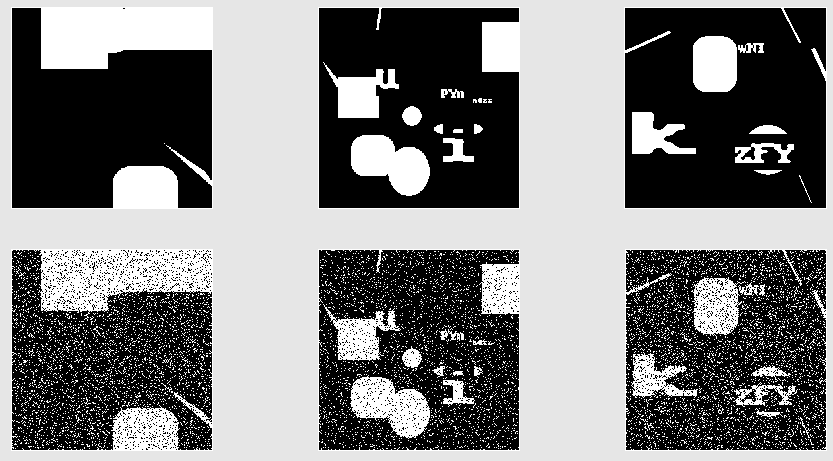
\includegraphics[scale=0.475]{binary_data_examples}
\caption{Examples of generated image pairs: ground-truth images (at the top) and observations (at the bottom).
The images on the left and in the center were generated with the noise level $\tilde{\alpha} = 0.1$, while the
images on the right were generated with the noise level $\tilde{\alpha} = 0.15$.}
\label{fig:binary_data_examples}
\end{figure}

\section{Denoising quality based on image size}

As part of our analysis, we have plotted the rate of convergence depending on the input resolution.\ The
results of the experiment are shown in \textit{Figure} \ref{fig:binary_input_size_plots}.\ In
both cases of $300{\times}300$ and $1000{\times}1000$ images, the noise level was set to $\tilde{\alpha} = 0.1$
and the observation strength was set to $1 - \alpha = 1 - \tilde{\alpha}$.\ As it is shown in the diagrams,
the gradient-based method converges to an original image within one hundred thousand steps.\ In contrast,
the Gibbs sampling method needs millions of iterations in order to converge to an original image.

\section{Denoising quality based on noise level}

In this section, we explore the impact of the noise level $\tilde{\alpha}$.\ In order to determine whether both
methods are able to reconstruct original images, we have run our experiments for
$\tilde{\alpha} \in \{0.05, 0.10, 0.15\}$ and set the observation strength $1 - \alpha = 1 - \tilde{\alpha}$.\ The
results of the analysis are shown in \textit{Figure} \ref{fig:binary_noise_level_plots}.\ From the presented
diagrams, it follows that both methods converge to the original images, even in the case of relatively high noise
level.\newline\newline\newline\newline

\begin{figure}[H]
\centering
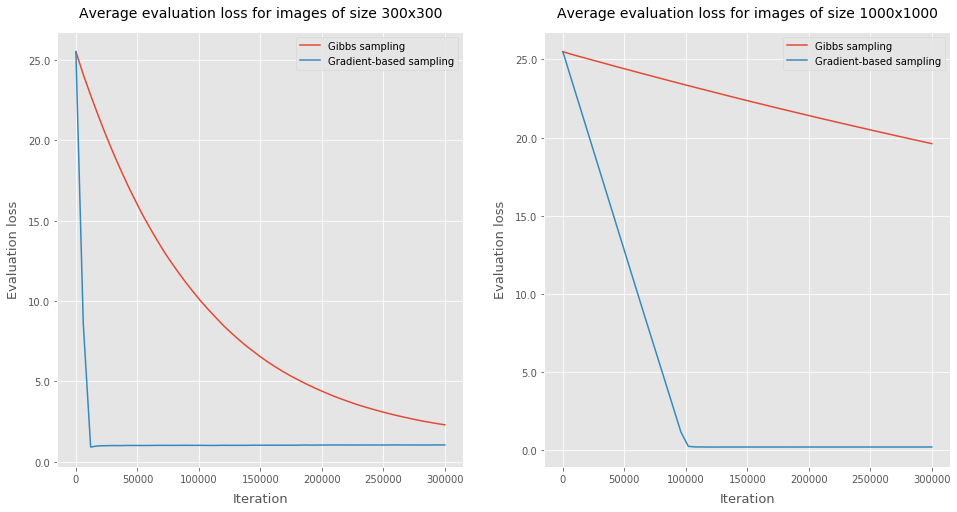
\includegraphics[scale=0.38]{binary_input_size_plots}
\caption{Comparison of the Gibbs sampling and our gradient-based method, based on input image size. The results
show that while the Gibbs algorithm needs millions of iterations in order to converge for $1000{\times}1000$ images, our
gradient-based method converges after roughly $100\ 000$ iterations.}
\label{fig:binary_input_size_plots}
\end{figure}

\begin{figure}[H]
\centering
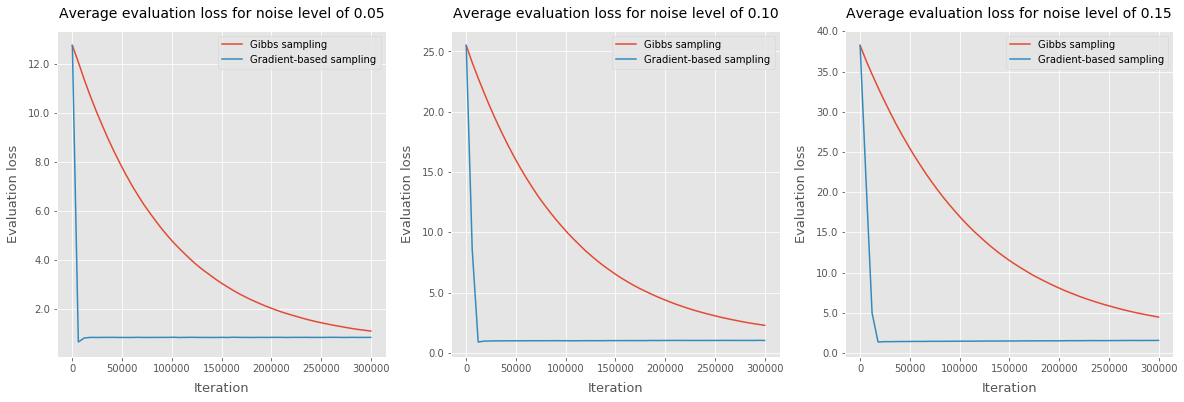
\includegraphics[scale=0.35]{binary_noise_level_plots}
\caption{Comparison of the Gibbs sampling and our gradient-based method, based on the noise level
$\tilde{\alpha}$. Both methods converge to the original images, regardless of the value of
the parameter $\tilde{\alpha}$.}
\label{fig:binary_noise_level_plots}
\end{figure}


\section{Sensitivity of the observation strength parameter}

In the previous sections, we leveraged the fact that the noise level $\tilde{\alpha}$ is known, by setting
the observation strength $1 - \alpha = 1 - \tilde{\alpha}$.\ In practical applications, it is often the case that
we observe an image without any hint how many pixels are flipped.\ In the present section,
we test different values of $\alpha \in \{0.01, 0.05, 0.15, 0.25, 0.35\}$, while keeping the value of the
noise level $\tilde{\alpha} = 0.05$ fixed.\ The results of our analysis are presented in
\textit{Figure} \ref{fig:binary_noise_level_prior_plots}, showing that our method estimates the original
image correctly even when the difference $|\alpha - \tilde{\alpha}|$ is high.

\begin{figure}[H]
\centering
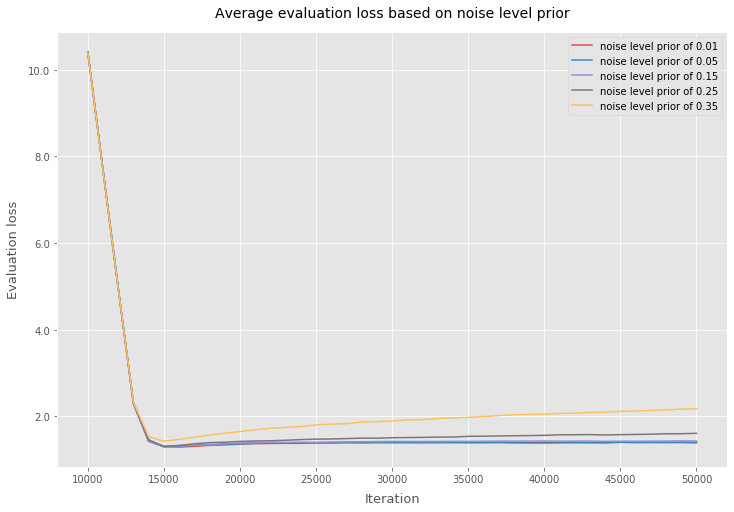
\includegraphics[scale=0.55]{binary_noise_level_prior_plots}
\caption{Comparison of the image reconstruction quality based on the observation strength $1 - \alpha$ for the
fixed noise level $\tilde{\alpha} = 0.05$. The $L_1$ errors are close $0.0$ in all cases expect for the cases of
$\alpha = 0.25$ and $\alpha = 0.35$ for which the errors are a bit higher, but still close to $0.0$. Interestingly,
in these two cases the quality degrades over time, suggesting that the optimization method has too
much flexibility.}
\label{fig:binary_noise_level_prior_plots}
\end{figure}

\section{Qualitative results}

The last conducted experiment involved comparing visual outputs produced by the Gibbs sampling and our
gradient-based method.\ To do so, we performed $100\ 000$ steps of both methods and converted the last states
of the simulated chains into images.\ The outcomes of this analysis are presented in \textit{Figure}
\ref{fig:binary_qualitative_results}.\ The results of this experiment confirm that our method is superior to
the Gibbs sampling method.\ In particular, it generated images that look identical to the original images,
even in dense text areas.\ Furthermore, the difference of quality between both methods is more visible for
high-resolution images as our method scales better to high-dimensional data than the Gibbs sampling
method.\newline\newline\newline\newline\newline\newline



\begin{figure}[H]
\centering
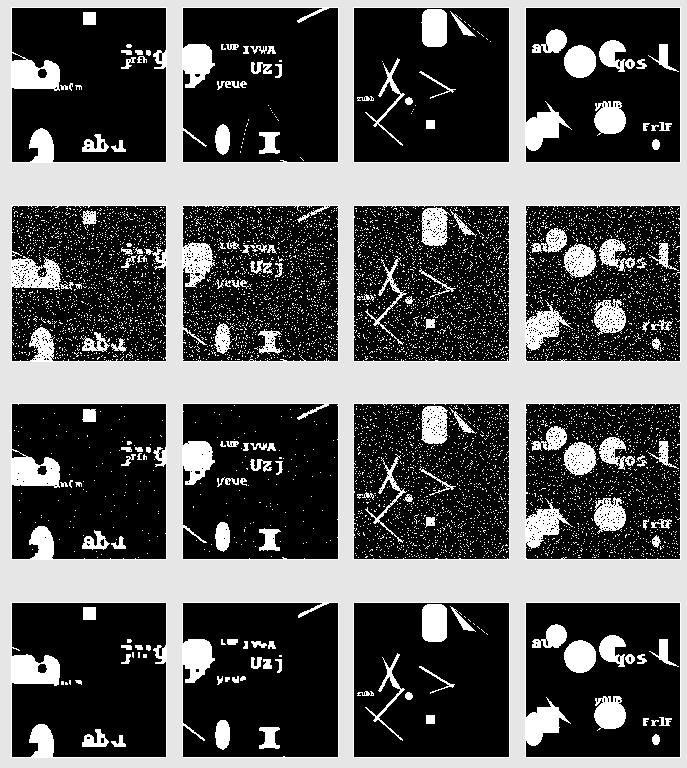
\includegraphics[scale=0.52]{binary_qualitative_results}
\caption{The comparison of the results generated by performing $100\ 000$ iterations of the discussed optimization
methods: original images (1st row), observed images (2nd row), images generated by the Gibbs
sampling method (3rd row) and our gradient-based method (4th row). While the images generated the Gibbs sampling
method contain quite a few noise pixels, our gradient-based method reconstructed the original images almost
perfectly. The images on the left side have a resolution of $300{\times}300$, while the images on the right side
have a resolution of $1000{\times}1000$.}
\label{fig:binary_qualitative_results}
\end{figure}

\numberedchapter{Experiments: grayscale images}\label{chapter:grayscale_experiments}

The problem of denoising grayscale images is more complex than the analogous problem for binary
images.\ Actually, the space of possible states is exponentially larger as each pixel can take $255$ different
values.\ In this chapter we will consider a model in which the noise is added to an original image by flipping
the values of random pixels.\ We will show that our method solves the stated problem in an effective manner
and present the results obtained on real photos.

\section{Methodology}

To run our experiments, we have collected $20$ grayscale photos and rescaled them to the fixed width of $800$,
keeping width-to-height aspect ratio of an original image.\ After rescaling, the collected images contain between
200,000 and 1,000,000 pixels.\ Then, for each photo we generated an observation $Z$ by applying
$$
Z_{ij} =
\begin{cases}
  255 - X_{ij} &\text{if $U_{ij} < \tilde{\alpha}$}\\
  X_{ij} &\text{otherwise}
\end{cases}\ ,
$$
where $U_{ij}$ is an i.i.d.\ sequence of $Unif(0, 1)$ random variables and $\tilde{\alpha} \in \{0.1, 0.2\}$ controls
the noise level.\ An example of an original photo along with its noisy versions is presented
in \textit{Figure} \ref{fig:grayscale_data_examples}.\ In order to measure the quality of reconstructed images,
we use already defined $L_1$ loss function
$$
L_1(\tilde{X}, X) = \sum\limits_{i = 1}^n \frac{|\tilde{X}_i - X_i|}{n}\ ,
$$
where $\tilde{X_i}, X_i \in \{0, 1,  \dots, 255\}$.\ As a result, it holds $L_1(\tilde{X}, X) \in [0,255]$, where 0
denotes the perfect prediction.\ The $L_1$ loss is averaged over all collected
photos.\newline\newline\newline\newline\newline

\begin{figure}[H]
\centering
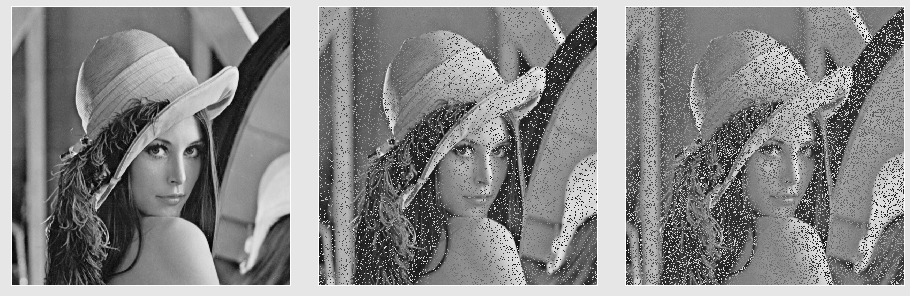
\includegraphics[scale=0.43]{grayscale_data_examples}
\caption{An example of real photo (on the left), the photo with the noise level $\tilde{\alpha} = 0.1$
(in the center), the photo with the noise level $\tilde{\alpha} = 0.2$ (on the right).}
\label{fig:grayscale_data_examples}
\end{figure}

\section{Denoising quality}

In order to determine whether our method is able to reconstruct original images, we performed the analysis with
$\tilde{\alpha} = 0.1$ and $\tilde{\alpha} = 0.2$ while comparing it with the Gibbs sampling method.\ We set
the observation strength $\alpha = \tilde{\alpha}$, nevertheless we observed that both optimization methods are not
sensitive to the value of this parameter and provide good estimations when $\alpha \neq \tilde{\alpha}$.\ The
results of our experiment are shown in \textit{Figure} \ref{fig:grayscale_noise_level_plots}.\ The first outcome
is that our method converges to an original image in two hundred thousand steps, fixing some corrupted pixel in each
iteration.\ Furthermore, the errors are close $0.0$, meaning that the estimations of our method are near
perfect.\ Lastly, the Gibbs sampling method also converges to an original image, but it needs several million
iterations to provide a good estimation.\newline

\begin{figure}[H]
\centering
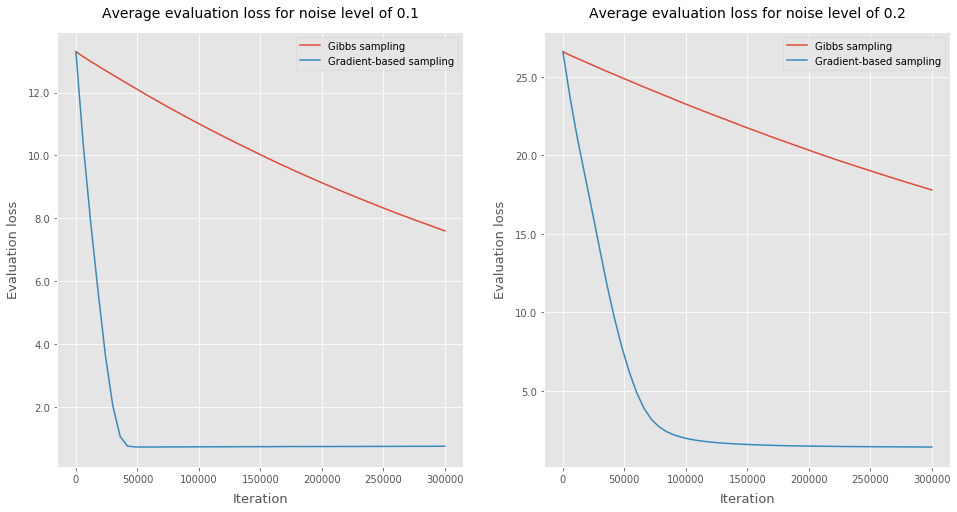
\includegraphics[scale=0.36]{grayscale_noise_level_plots}
\caption{Comparison of the Gibbs sampling and our gradient-based method, based on the noise level
$\tilde{\alpha}$. The results show that while both methods converge to the original images, our method generates
near-perfect estimation of an original image in relatively small number of steps}
\label{fig:grayscale_noise_level_plots}
\end{figure}

\section{Qualitative results}

In this section we present the visual comparison of images generated by the Gibbs sampler and our method.\ Like
in the case of binary images, we performed $100\ 000$ iterations of the discussed methods and converted the last
simulated states into images.\ The results of this analysis are shown in \textit{Figure}
\ref{fig:grayscale_qualitative_results}, proving that our method is able to reconstruct images in relatively
small number of steps.\ Particularly, our method reconstructed all $20$ images almost perfectly, while the
results generated by the Gibbs sampler were very noisy.\newline

\begin{figure}[H]
\centering
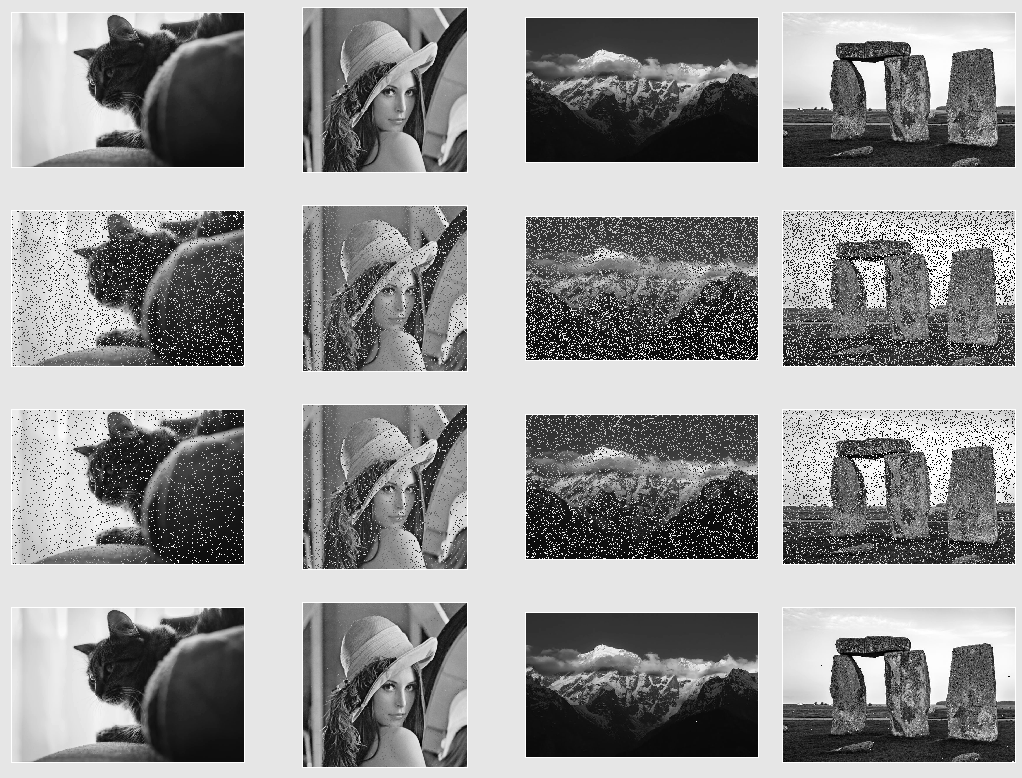
\includegraphics[scale=0.385]{grayscale_qualitative_results}
\caption{The comparison of the results generated after $100\ 000$ iterations of the discussed image denoising
methods: original images (1st row), observed images (2nd row), images generated by the Gibbs
sampling method (3rd row) and our gradient-based method (4th row). While the results obtained with the Gibbs
sampling method are very noisy, our reconstruction method generated images with hardly any corrupted pixels. The
images on the left side were generated with the noise level $\tilde{\alpha} = 0.1$, while the images on the right
side were generated with the noise level $\tilde{\alpha} = 0.2$.}
\label{fig:grayscale_qualitative_results}
\end{figure}

\numberedchapter{Summary}

In this thesis we have shown how a seemingly unrelated
problem of image denoising can be rephrased in a way that allows the discussed Markov chain Monte Carlo methods to be
applied.\ As the first step of our analysis, we have identified the main downside of the classical Gibbs sampling
algorithm in the context of the considered problem.\ Then, we have developed gradient-based approach that is designed
to optimize pixels making up the best candidates to update.\ Additionally, we have implemented an algorithm that
performs one step of the developed method in the time complexity $\mathcal{O}(1)$.\ During our experiments we have
shown that our approach actually outperforms the Gibbs sampling algorithm.\ In particular, the conducted analysis
clearly showed that the developed approach can scale to multi-million dimensional spaces, while it is not the case for
the Gibbs sampling algorithm.\ Besides it, we proved that our method is not sensitive to the observation strength
parameter, which makes it possible to apply it even when the noise level is unknown.\ Finally, we have
successfully extended our approach to the case where some pixels of a grayscale image are flipped.\ Particularly,
our method provided impressing results on noisy photos, generating near-perfect reconstructions.\newline

\noindent Although we have conducted many experiments of our method, there is still much room for further
extensions.\ For instance, one may extend our algorithm to denoise grayscale images that are
generated by adding random perturbations.\ The other practical application is to tackle the problem of
denoising \textit{RGB} images.\ Lastly, our algorithm can be applied to other problems than image denoising.


\begin{thebibliography}{9}

\bibitem{markov_chains_book}
O. Häggström - \textit{Finite Markov chains and algorithmic applications. Cambridge University
Press; 1st edition (2002)}

\bibitem{mcmc_book}
P. Bremaud - \textit{Markov chains: Gibbs Fields, Monte Carlo Simulation, and Queues. Springer-Verlag New
York (1999)}

\bibitem{oops_gradient}
W. Grathwohl, K. Swersky, M. Hashemi, D. Duvenaud, C. Maddison -
\textit{Oops I Took A Gradient: Scalable Sampling for Discrete Distributions. Link to arXiv paper:
\url{https://arxiv.org/pdf/2102.04509.pdf} (2021)}

\end{thebibliography}

\end{document}
